\section{The Reward Problem}
% The day's spine
\begin{frame}{The Reward Problem Has Three Faces}
\begin{itemize}
    \setlength{\itemsep}{0.7em}
    \item \textbf{We have the reward, but where is it?}\\
          \emph{Exploration vs.\ exploitation} --- bandits, UCB, Thompson sampling, curiosity (today).
    \item \textbf{The reward we wrote is wrong.}\\
          \emph{Reward shaping \& specification gaming} (today).
    \item \textbf{We can't write a reward at all.}\\
          \emph{Inverse RL \& preference-based reward learning} (today --- and the direct ancestor of RLHF on Day 9).
\end{itemize}
\vspace{0.6em}
\centering\small\textcolor{gray}{One day, three faces of the same problem.}
\end{frame}

% --- Exploration vs Exploitation, split into 2 ---
\begin{frame}{Exploration vs.\ Exploitation: The Dilemma}
\begin{itemize}
    \setlength{\itemsep}{0.5em}
    \item Many situations in business (\& life!) present a dilemma between two kinds of choices
    \item \textbf{Exploitation:} pick choices that seem best based on past outcomes
    \item \textbf{Exploration:} pick choices not yet tried (or not tried enough)
    \item Exploitation has notions of ``being greedy'' and being ``short-sighted''
    \item Exploration has notions of ``gaining information'' and being ``long-sighted''
\end{itemize}
\end{frame}

\begin{frame}{Exploration vs.\ Exploitation: The Trade-Off}
\begin{itemize}
    \setlength{\itemsep}{0.6em}
    \item Too much \emph{exploitation} $\Rightarrow$ regret of missing unexplored ``gems''
    \item Too much \emph{exploration} $\Rightarrow$ regret of wasting time on ``duds''
    \item How do we balance them to combine information-gains with greedy-gains in the most efficient manner?
    \item \textcolor{red}{Can we set this up in a mathematically disciplined manner?} $\to$ next sections
\end{itemize}
\end{frame}

\begin{frame}{Examples}
\begin{itemize}
    \item Restaurant Selection
    \begin{itemize}
        \item Exploitation: go to your favorite restaurant
        \item Exploration: try a new restaurant
    \end{itemize}
    \item Online Banner Advertisement
    \begin{itemize}
        \item Exploitation: show the most successful advertisement
        \item Exploration: show a new advertisement
    \end{itemize}
    \item Oil Drilling
    \begin{itemize}
        \item Exploitation: drill at the best known location
        \item Exploration: drill at a new location
    \end{itemize}
    \item Learning to play a game
    \begin{itemize}
        \item Exploitation: play the move you believe is best
        \item Exploration: play an experimental move
    \end{itemize}
\end{itemize}
\end{frame}

\section{The Multi-Armed Bandit Problem}
% --- MAB problem, split into 2 ---
\begin{frame}{The Multi-Armed Bandit (MAB) Problem}
\begin{itemize}
    \setlength{\itemsep}{0.45em}
    \item ``Multi-Armed Bandit'' is a tongue-in-cheek name for ``many single-armed bandits'' --- a row of slot machines
    \item Formally, a 2-tuple $(\mathcal{A}, \mathcal{R})$
    \begin{itemize}
        \item $\mathcal{A}$: a known set of $m$ actions (``arms'')
        \item $\mathcal{R}^a(r) = \mathbb{P}[r \mid a]$: an \emph{unknown} reward distribution for each arm
    \end{itemize}
    \item At each step $t$, the agent selects an action $a_t \in \mathcal{A}$ and the environment generates a reward $r_t \sim \mathcal{R}^{a_t}$
\end{itemize}
\end{frame}

\begin{frame}{The Goal: Maximize Cumulative Reward}
\begin{itemize}
    \setlength{\itemsep}{0.6em}
    \item The agent's goal: maximize the cumulative reward over $T$ steps
    \[
        \sum_{t=1}^{T} r_t
    \]
    \item \textbf{Can we design a strategy that does well (in expectation) for any $T$?}
    \item Every strategy walks a tightrope: \emph{wasting time on duds} while exploring, vs.\ \emph{missing untapped gems} while exploiting
\end{itemize}
\end{frame}

% --- MAB as MDP, split into 3 (view 1 / view 2 / big-picture) ---
\begin{frame}{Is the MAB Problem a Markov Decision Process? (1/2)}
\begin{itemize}
    \setlength{\itemsep}{0.55em}
    \item The environment doesn't have a notion of state --- pulling an arm just samples from a distribution
    \item But the \emph{agent} might maintain a statistic of history as its own state
    \item The action is then a (policy) function of this agent-state
    \item So the agent's arm-selection strategy is \emph{a policy} --- the MAB can be viewed as a (degenerate) MDP
\end{itemize}
\end{frame}

\begin{frame}{Is the MAB Problem a Markov Decision Process? (2/2)}
\begin{itemize}
    \setlength{\itemsep}{0.55em}
    \item In practice, most MAB algorithms \emph{don't} take this formal MDP view
    \item Instead, they rely on heuristic methods that don't aim to optimize the full MDP
    \item They simply strive for ``good'' cumulative rewards in expectation
    \item Even in the simplest heuristics, $a_t$ is a random variable --- it's a function of the past (random) rewards
\end{itemize}
\end{frame}

\begin{frame}{Big Picture: Bandits Are MDPs in Disguise}
\begin{center}
\renewcommand{\arraystretch}{1.5}
\large
\begin{tabular}{ll}
A bandit             & $=$ a \emph{one-state} MDP \\
A contextual bandit  & $=$ a \emph{one-step} MDP \\
Tomorrow's full RL   & $=$ the \emph{multi-step} case \\
\end{tabular}
\end{center}
\vspace{0.8em}
\begin{itemize}
    \item So everything we derive today \emph{lifts} to MDPs --- a bridge we'll revisit at the end of the lecture.
\end{itemize}
\end{frame}

\section{Regret}
\begin{frame}{Regret: The Language for ``Doing Well''}
\begin{itemize}
    \item The Action Value $Q(a)$ is the (unknown) mean reward of action $a$:
    \[
        Q(a) = \mathbb{E}[r \mid a]
    \]
    \item The Optimal Value $V^*$ is the best of these:
    \[
        V^* = Q(a^*) = \max_{a \in \mathcal{A}} Q(a)
    \]
    \item \textbf{Single-step Regret} $l_t$ is the opportunity loss at step $t$:
    \[
        l_t = \mathbb{E}[V^* - Q(a_t)]
    \]
    \item \textbf{Total Regret} $L_T = \sum_{t=1}^{T} l_t$
    \item Maximizing cumulative reward $\;\equiv\;$ minimizing total regret
\end{itemize}
\end{frame}

\begin{frame}{Counting Regret: Counts and Gaps}
\begin{itemize}
    \setlength{\itemsep}{0.5em}
    \item Let $N_t(a) = $ number of times $a$ has been selected by step $t$
    \item Let $\Delta_a = V^* - Q(a)$ be the \emph{gap} between action $a$ and the optimal action
    \item Then total regret decomposes cleanly:
    \[
        L_T \;=\; \sum_{a \in \mathcal{A}} \mathbb{E}[N_T(a)] \cdot \Delta_a
    \]
    \item \textcolor{red}{A good algorithm ensures small counts for large gaps}
    \item \emph{Catch:} we don't know the gaps in advance --- they're properties of the unknown reward distribution
\end{itemize}
\end{frame}

\begin{frame}{Linear or Sublinear Total Regret?}
\centering
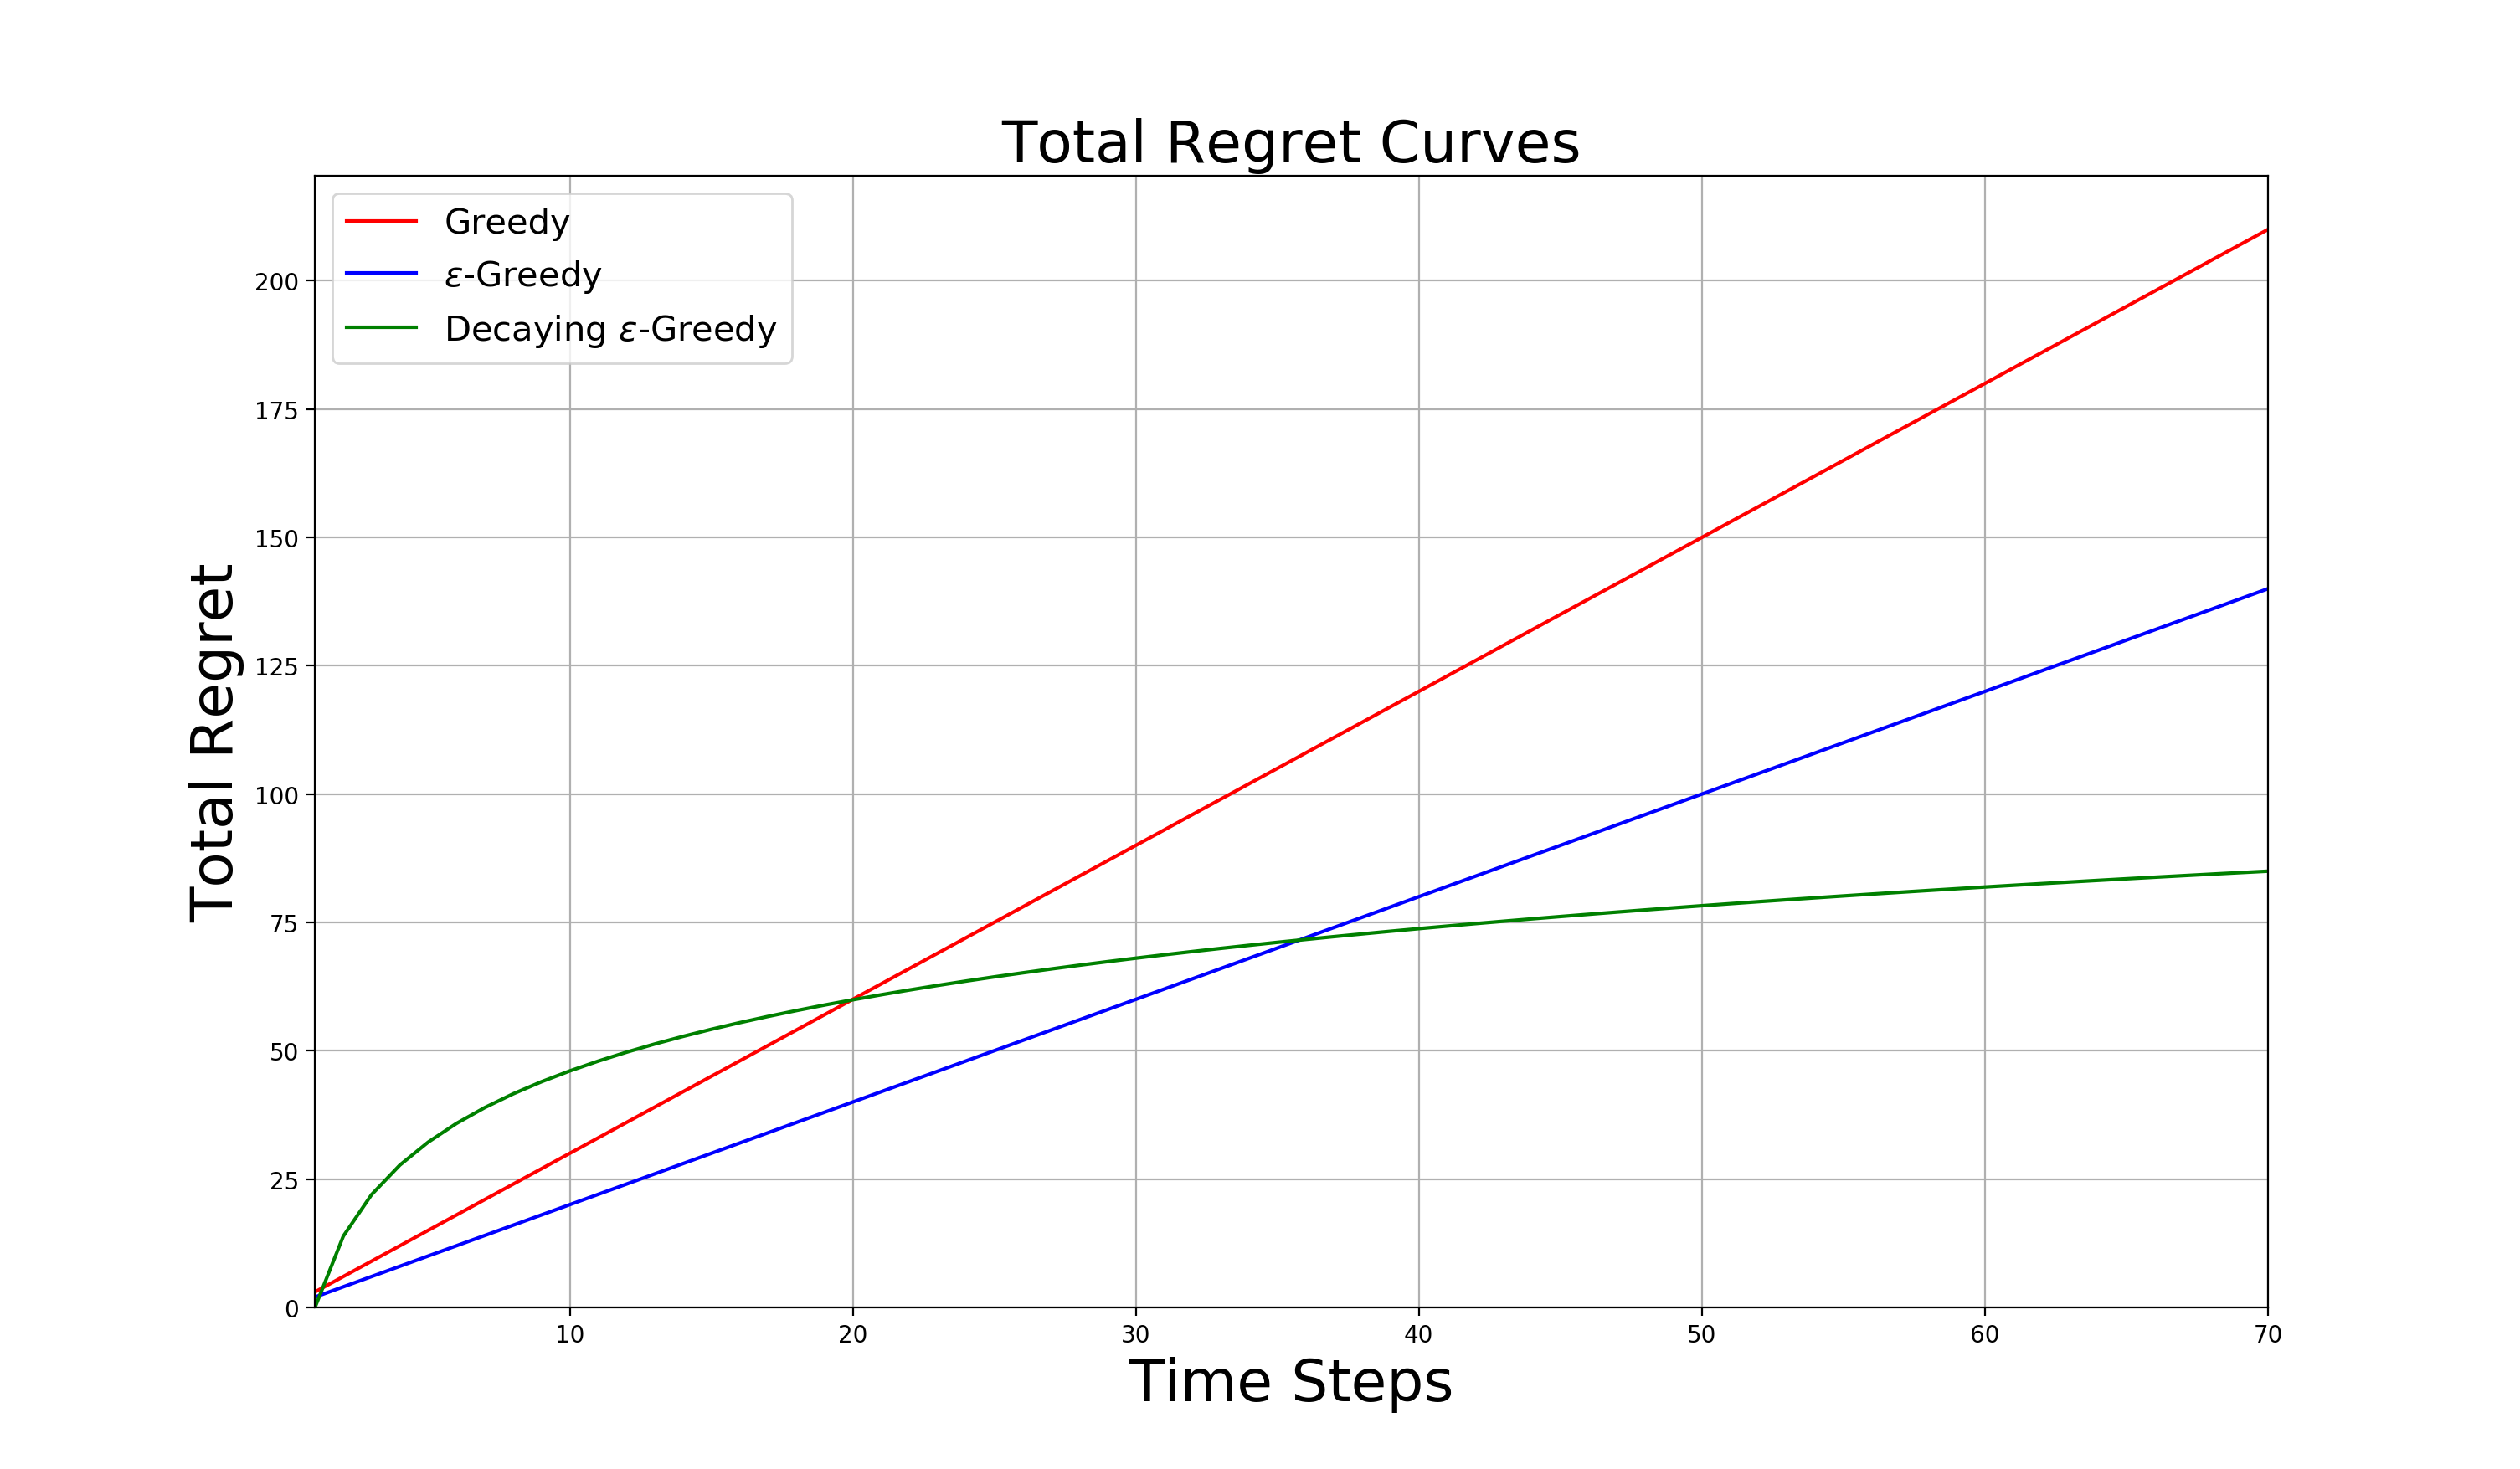
\includegraphics[width=0.58\textwidth,height=0.55\textheight,keepaspectratio]{images/bandits/figures/regret-curves.jpg}
\begin{itemize}
    \item If an algorithm \emph{never} explores $\Rightarrow$ linear total regret
    \item If an algorithm \emph{forever} explores $\Rightarrow$ linear total regret
    \item \textbf{Is sublinear total regret achievable?} (Spoiler: yes.)
\end{itemize}
\end{frame}
